\chapter{Definition B-Baum}

Ein B-Baum ist ein balancierter Suchbaum der Ordnung $n$, wenn es folgende Eigenschaften enth\"alt:

	\begin{enumerate}
		\item Jeder Knoten besitzt mindestens $1$ und h\"ochstens $n-1$ Elemente.
		\item Jeder Knoten mit $m$ Elemente hat $m+1$ S\"ohne, au\ss er Bl\"atter.
		\item Jeder Wert der Elemente im linken Teil des Baumes ist kleiner als die Werte des rechten Teil des Baumes.
		\item Alle Bl\"atter m\"ussen die gleiche Tiefe $h$ haben und d\"urfen keinen Nachfolger geben.
	\end{enumerate}
Nehmen wir einen B-Baum der Ordnung $3$ als Beispiel(siehe Abb. \ref{d1}). Jeder Knoten dieses Baumes kann zwischen 1 und 3 Elemente haben. Ein innere Knoten hat im unseren Beispiel 3 S\"ohne. Die Werten der Elemente erh\"ohen sich vom linken Teil bis zum rechten Teil des Baumes. Dazu kommt noch, dass jedes Blatt die gleiche Tiefe hat. Im diesen Fall hat jedes Blatt die Tiefe $3$.
Somit stimmen alle oben genannten Eigenschaften \"uberein.
\begin{figure}[h!] %[hbtp]
	\centering
		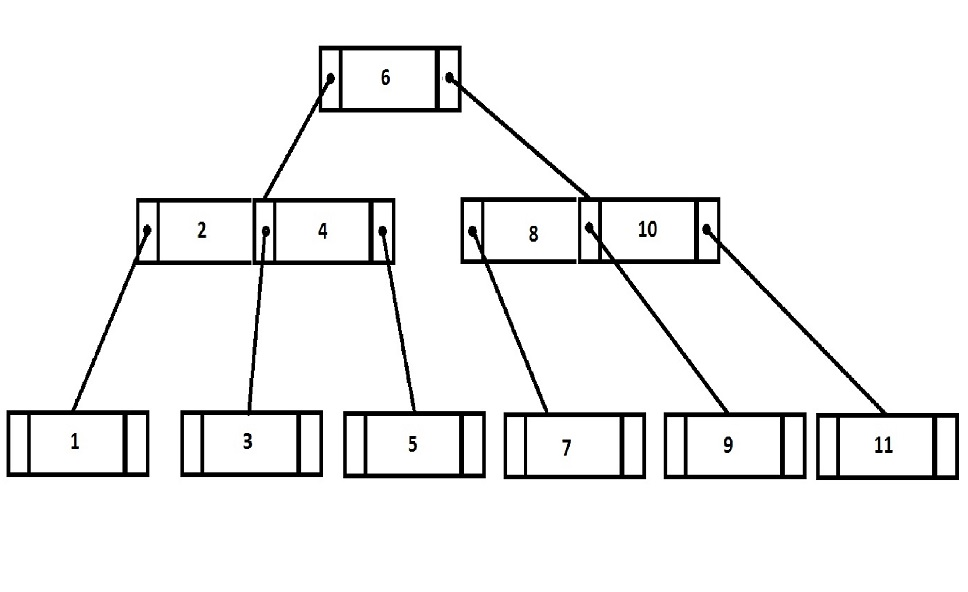
\includegraphics[scale=0.5]{images/definition.jpg}
	\caption{Beispiel eines B-Baumes}
	\label{d1}
\end{figure}

\paragraph{}
Es gibt ein spezieller B-Baum, der $1$,$2$ oder $3$ Elemente pro Knoten hat und $2$, $3$ oder $4$ S\"ohne haben kann. Dieser Baum wird als 2-3-4-Baum gekennzeichnet(siehe Abb. \ref{b234}).
\begin{figure}[h!] %[hbtp]
	\centering
		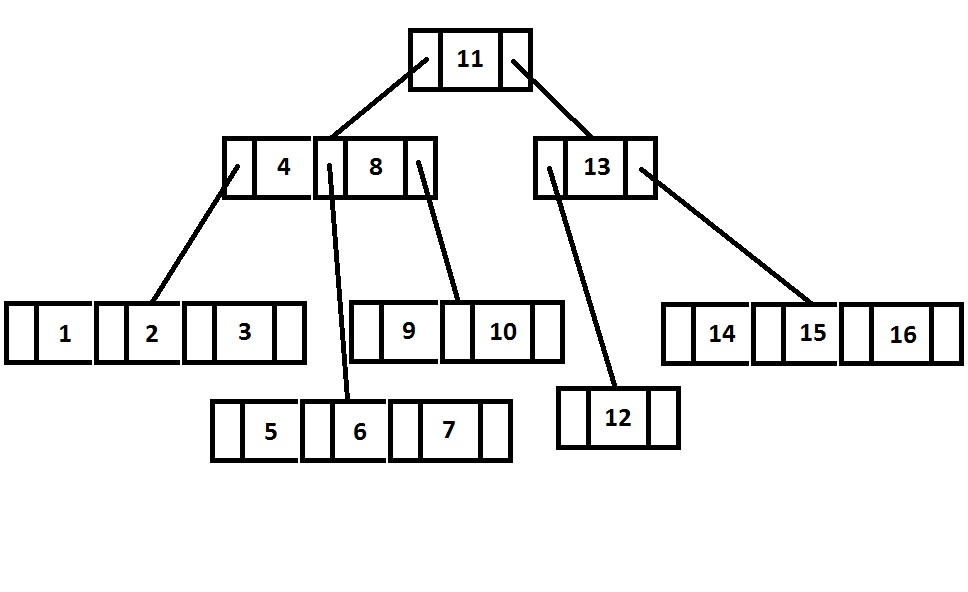
\includegraphics[scale=0.5]{images/234baum.jpg}
	\caption{2-3-4-Baum}
	\label{b234}
\end{figure}